 Dans cette partie, nous utiliserons des simulations turbulentes issues de deux modèles décrivant des anisotropies de pression, le premier dépend d'une fermeture \cacro{CGL} tandis que le second dépend d'une fermeture de type \cacro{LF}. Ces modèles sont simulés avec un seul et unique code que l'on va présenter dans ce chapitre. Les spécificités des modèles seront détaillées dans les Chapitres \ref{ch-33} et \ref{ch-34}. Dans ce premier chapitre, seront abordées les méthodes numériques utilisées dans l'implémentation de ces modèles (section \ref{sec-311}) ainsi que la description des méthodes de post-traitement associées au calcul des lois exactes (section \ref{sec-312}) et à leur visualisation (section \ref{sec-313}). Les valeurs des paramètres décrits dans la section \ref{sec-311} sont résumés dans la \tabref{tab:setups} et la \tabref{tab:setups_hd} pour chaque simulation.
 

\section{Simuler un plasma turbulent }
\label{sec-311}

 Le code de simulation utilisé, codé en \verb|Fortran|, est un code tridimensionnel pseudo-spectral et versatile développé en interne à l'Observatoire de la Côte d'Azur pour l'implémentation du modèle fluide proposé par \cite{snyder_landau_1997} et étendu par [\cite{goswami_landau_2005}, \cite{passot_collisionless_2007}, \cite{passot_extending_2012}, \cite{sulem_landau_2015}]. Ce modèle prend en compte les termes gyrotrope et non-gyrotrope des tenseurs de pression des ions et des électrons et capte l'effet Landau ionique et électronique à travers les flux de chaleur des électrons et des ions. Le code permet à l'utilisateur de choisir quelles contributions garder.
 
 Les quantités sont sans dimension, les longueurs sont normalisées par $d_i$, la longueur inertielle des ions, et les vitesses par la vitesse d'Alfvén. Cela induit une constante $\beta/2$, avec $\beta = 1$, présente dans tous les termes dépendant des pressions. Il faudra prendre en compte cette constante par la suite. 
 
  Supposons une équation générique $\partial_t X = \boldsymbol{v} \cdot \nabla  X$. La simuler via un code pseudo-spectral (algorithme schématisé sur la \figref{fig:algo_OCA}) signifie que les dérivées spatiales telles que $\nabla X$ sont effectuées dans l'espace de Fourier, tandis que les produits tels que $\boldsymbol{v} \cdot \nabla  X$  et l'intégration temporelle de l'équation pour obtenir les quantités au pas de temps suivant, sont effectués dans l'espace réel. Ainsi, à chaque pas de temps, un aller-retour est effectué entre les espaces réel et de Fourier. Leur discrétisation en un nombre de points finis, ou grille numérique, induit un repliement du spectre, dit \og aliasing \fg{}, des termes non-linéaires. Cet effet est limité par une troncation à chaque pas de temps du spectre de chaque quantité. L'intégration temporelle est obtenue via un \cacro{RK3}, choisi pour sa stabilité devant des termes dispersifs tels que le terme de \cacro{Hall} [\cite{williamson_low-storage_1980}]. Les conditions de bords de la grille numérique sont choisies comme périodiques afin de pouvoir utiliser la transformation de Fourier et l'\cacro{FFT}. 
 \begin{figure}[!ht]
 \centering
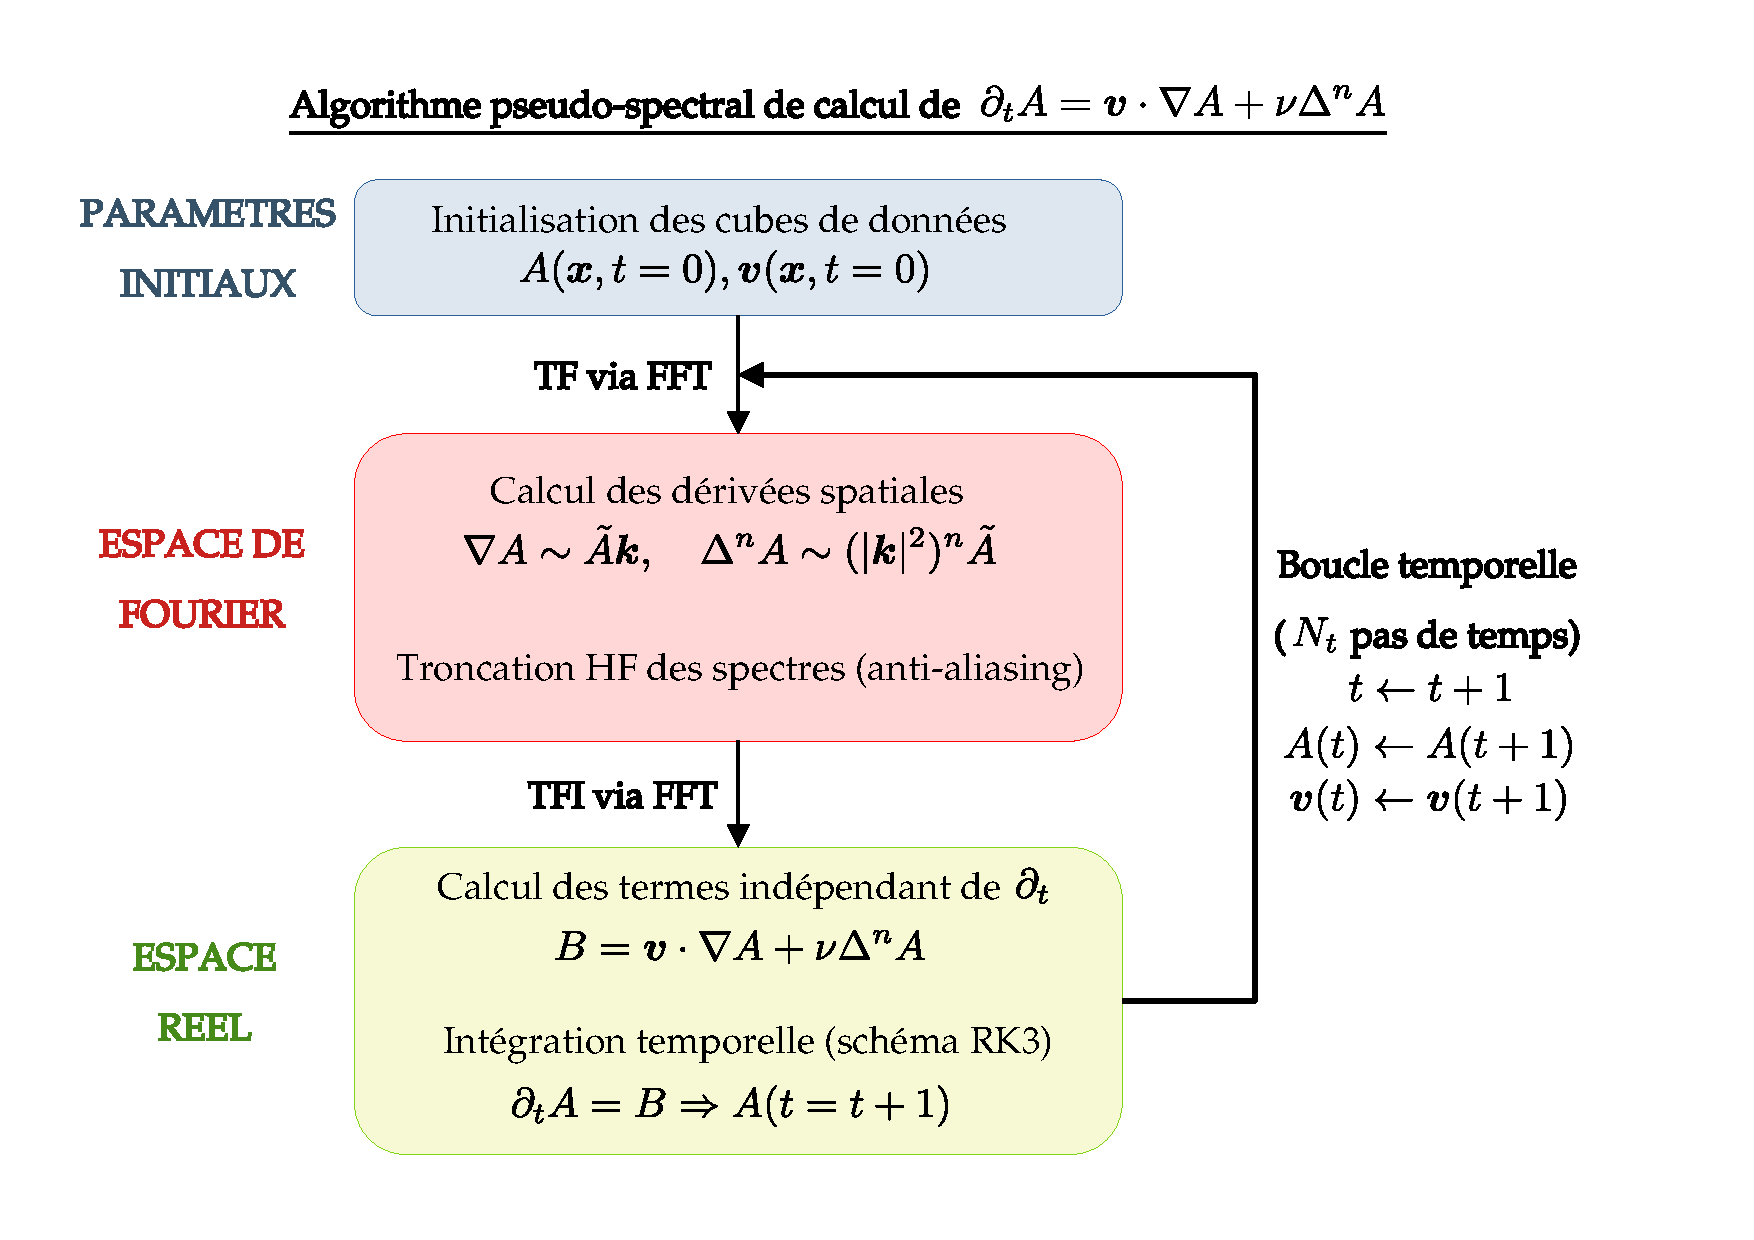
\includegraphics[width=0.9\linewidth,trim=1cm 1cm 3cm 1cm, clip=true]{./Mainmatter/Part_3/images_ch1/code_OCA}
\cprotect\caption{Algorithme d'intégration d'une équation d'évolution générique via une méthode pseudo-spectrale. Prise en compte des corrections d'anti-aliasing et d'hyperdissipation \ensuremath{\nu \Delta^n A}. TF(I) correspond à transformée de Fourier (inverse). }
\label{fig:algo_OCA}
\end{figure}

 Afin de limiter l'apparition de fort gradients et autres discontinuités liées à des instabilités numériques et induisant un arrêt brusque de la simulation, deux possibilités existent : appliquer un filtre passe-bas sur le spectre de la quantité impliquée ou un terme d'hyperviscosité dans son équation. Le choix effectué est celui de l'hyperviscosité, c'est-à-dire imposer une décroissance graduelle et de plus en plus intense du spectre de la quantité (pour plus d'informations, se référer à [\cite{borue_forced_1995,frisch_hyperviscosity_2008}]). Ce terme de dissipation numérique s'écrit $\nu \Delta^{n} X$ pour un champ $X$, avec $\nu$ une constante choisie initialement et $n$ un entier fixé à 4. $\Delta^{n}$ est effectué dans l'espace de Fourier où une décroissance du spectre en $\boldsymbol{k}^{-8}$ est donc obtenue.   
 L'existence d'un champ magnétique moyen dans les simulations induit une anisotropie spatiale de la turbulence. Sa direction est imposée suivant $\boldsymbol{e_z}$. Afin de refléter cette anisotropie, l'hyperviscosité est adaptée avec un paramètre $\alpha$ : $\Delta^{n}$ est calculé dans l'espace de Fourier tel que $(k^2_x +  k^2_y + \alpha k^2_z)^n$. Les paramètres $\nu$ et $\alpha$ sont résumés dans la \tabref{tab:setups_hd}. Avec le pas de temps $\delta t$, ils sont accordés empiriquement afin de réduire le temps de calcul, de maintenir la dissipation aux vecteurs d'onde les plus grands et d'éviter tout emballement de la simulation et l'apparition d'instabilités numériques. En termes de turbulence, l'hyperviscosité sera considérée comme le terme de dissipation évacuant l'énergie aux petites échelles.
 
 La cascade d'énergie est entretenue par un forçage permanent\footnote{Dans [\cite{hellinger_von_2018}, \cite{gomez_parallel_2005}, \cite{mininni_hybrid_2011}], une autre méthode est utilisée pour obtenir le développement d'une cascade turbulente : leurs champ de vitesse et champ magnétique sont initialisés par une superposition de modes de phases aléatoires, puis leurs simulations évoluent librement (simulations en déclin).}. Ce forçage de type antenne de Langevin (oscillateur harmonique forcé aléatoirement [\cite{tenbarge_oscillating_2014}]) injecte la somme de deux ondes de fréquences aléatoires mais proches de celle de l'onde d'Alfvén cinétique avec une amplitude correspondand au paramètre $A_f$ multiplié par un facteur aléatoire. Il est  
appliqué sur le champ de vitesse de sorte à maintenir la somme des énergies cinétique et magnétique perpendiculaires moyennes sous un niveau $E_{sup}$ et au-dessus d'un niveau $E_{inf}$ proche de $E_{sup}$. L'énergie moyenne totale est donc quasi-constante. 
Dans l'espace de Fourier, il prend la forme d'un peigne de distributions de Dirac non nulles aux vecteurs d'ondes les plus petits, tels que $\boldsymbol{k} = \{(0,\pm 1, \pm 1);(\pm 1,\pm 1, \pm 1)\}$ dans la grille numérique associée à l'espace de Fourier. L'angle d'injection de l'énergie, $\theta_i$, sert à définir la forme de la grille spatiale, un parallélépipède allongé dans la direction $\boldsymbol{e_z}$, la taille physique de cette grille est fixée telle que $L_{\perp}/L_z = \tan \theta_i$ avec $L_{\perp} = \frac{2 \pi}{k_{0\perp}} $.
 
 La taille de l'espace des échelles accessibles via ces simulations dépend de la taille de la grille spatiale. L'échelle la plus petite dans une direction est la distance minimale entre deux points de la grille dans cette direction, et l'échelle la plus grande est la moitié de la taille de la grille. Pour une étude de turbulence, on a besoin de plusieurs ordres de grandeur entre les échelles minimales et maximales. Afin d'obtenir un nombre de points suffisant, on part d'une grille de taille physique fixée mais contenant peu de points, par exemple $128^3$, puis, après avoir atteint un régime turbulent satisfaisant tel que les spectres soient stabilisés, on augmente le nombre de points et ainsi de suite jusqu'à avoir la taille voulue pour l'espace des échelles et un spectre stable. Le nombre de points idéal serait $1024^3$ ou plus, mais plus il y a de points, plus le temps de calcul augmente\footnote{Typiquement, il faut environ un mois de calcul avec $64$ processeurs pour obtenir une simulation de taille $512^2\times 1024$ dans laquelle la turbulence se serait a priori entièrement développée} et plus le calcul monopolisera de la mémoire. Similairement, le calcul du taux de cascade sera aussi plus contraignant. Un compromis doit donc être trouvé. La taille de cube minimale considérée dans le cadre des études de turbulence sera $512^3$ et une partie des simulations aura une résolution de $512^2$ dans le plan $\{\boldsymbol{e_x},\boldsymbol{e_y}\}$ et $1024$ dans la direction $\boldsymbol{e_z}$. 
 
 Les simulations utilisées et détaillées dans la \tabref{tab:setups} et la \tabref{tab:setups_hd} ont, pour la plupart, fait l'objet de l'article [\cite{ferrand_fluid_2021}]. Parmi elles, une est de résolution $1024^3$. Elle ne sera pas traitée ici car sa taille est trop importante pour le code de post-traitement implémenté et les moyens de calcul à disposition (mésocentre). 
 
 \section{Code de post-traitement pour le calcul numérique de lois exactes }
 \label{sec-312}
 
 On a vu qu'une loi exacte est une formule statistique donnant un résultat en fonction de l'échelle $\boldsymbol{\ell}$. Elle dépend de quantités évaluées localement en deux points puis combinées en une expression qui est ensuite moyennée. Une partie des termes doit ensuite être dérivée dans l'espace des échelles si aucune hypothèse d'intégration n'est effectuée. Cette méthode pourrait être implémentée directement. On considèrerait les quantités à disposition, a priori des cubes évalués en $\boldsymbol{x}$), on les translaterait de sorte à obtenir des cubes évalués en $\boldsymbol{x} - \boldsymbol{\ell}$, puis on les combinerait suivant l'expression voulue avant de les moyenner. On obtiendrait ainsi notre résultat évalué en un point de l'espace des échelles et il faudrait recommencer encore et encore afin d'obtenir l'ensemble de l'espace des échelles. Enfin, on dériverait ou intégrerait le résultat. Cet algorithme est schématisé sur la \figref{fig:algo_direct}.
 \begin{figure}[!ht]
  \centering
 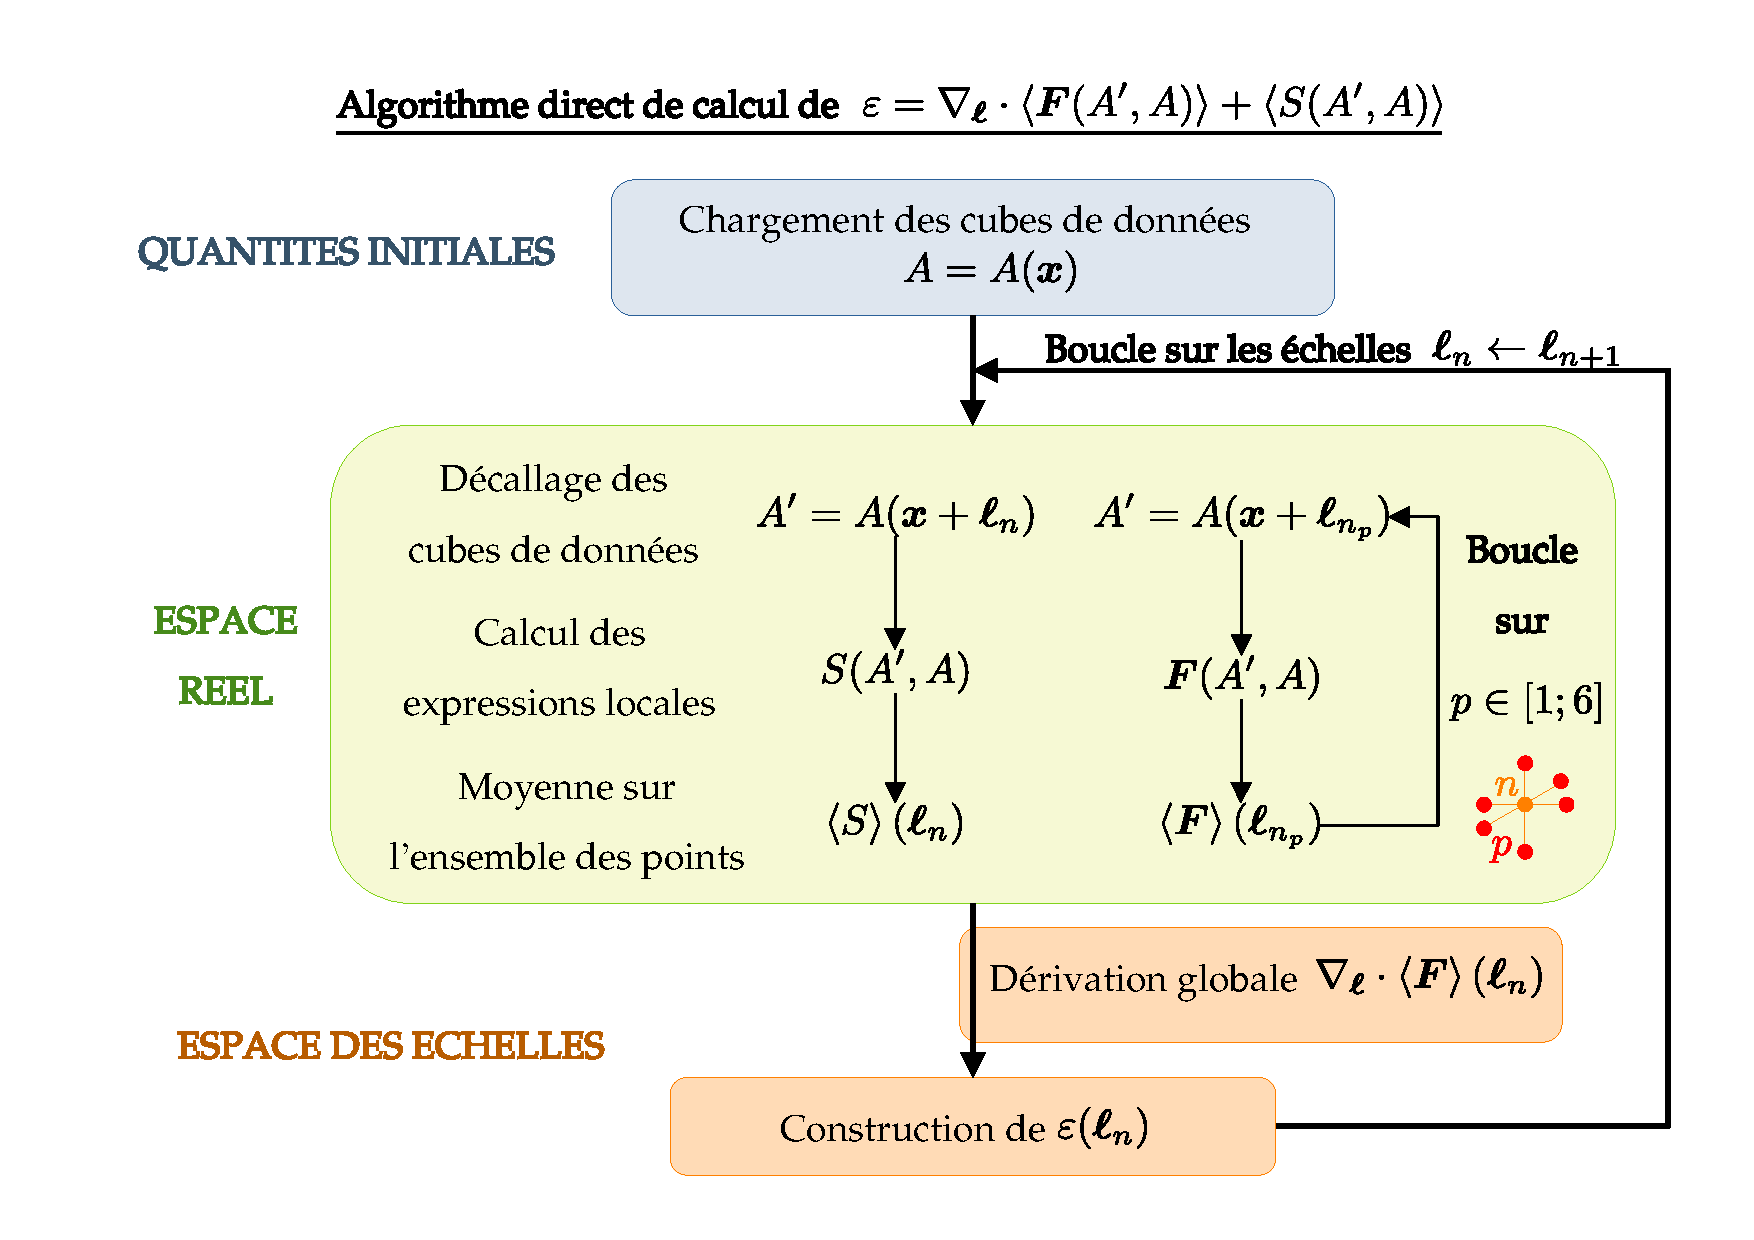
\includegraphics[width=0.9\linewidth,trim=2cm 1cm 1cm 1cm, clip=true]{./Mainmatter/Part_3/images_ch1/code_EL_direct}
 \cprotect\caption{Algorithme de calcul du taux de cascade \ensuremath{\varepsilon} via la méthode directe. Les quantités impliquées sont des quantités génériques.}
 \label{fig:algo_direct}
 \end{figure}
 
 Cette méthode est coûteuse en temps de calcul et demande des compromis. Pour réduire le temps de calcul, on peut choisir intelligemment un certain nombre de vecteurs d'échelle. Tout d'abord, on peut jouer sur la parité de la loi exacte et ne calculer que les vecteurs tels que $\ell_z \leq 0$.  \cite{ferrand_fluid_2021} et \cite{ferrand_-depth_2022} par exemple, utilisent les hypothèses d'isotropie ou d'axisymétrie de l'espace d'échelles. Dans le cas isotrope, l'espace des échelles est alors vu comme une sphère avec 73 vecteurs directeurs partant de son centre. Dans le cas axisymétrique, le découpage est similaire, mais effectué dans des disques pour chaque $\ell_z$. La divergence dans l'espace des échelles est ensuite effectuée sphériquement (resp. cylindriquement) le long de $\ell = |\boldsymbol{\ell}|$ (resp. $\ell_{\perp} = \sqrt{\ell^2_x + \ell^2_y}$) en supposant les dérivées angulaires nulles. Je n'ai pas voulu faire de même, n'étant pas convaincue de l'indépendance angulaire de la dérivée et trouvant la statistique finale faible. Une autre possibilité est de choisir les vecteurs en fonction du mode de représentation final. Si ce mode de représentation est logarithmique, on peut ne choisir qu'un nombre limité de vecteurs à grande échelle tels qu'ils soient régulièrement espacés en représentation logarithmique [\cite{manzini_local_2022}]. Un problème de cette méthode est l'irrégularité de la grille résultante. La divergence dans l'espace des échelles doit donc se faire vecteur par vecteur à partir des six échelles les plus proches (au minimum). Ce choix-là ne semblait toujours pas satisfaisant, car il implique de devoir potentiellement refaire le calcul en fonction du mode de représentation final et un biais apparaît en cas de moyenne dans l'espace des échelles. Ces compromis doivent en plus être accompagnés d'une optimisation, voire d'une parallélisation du calcul numérique. 
 
 Après maintes versions et tentatives d'optimisation de mon code de post-traitement, codé en \verb|Python| et essayant de respecter explicitement la forme de la loi exacte, j'ai décidé de changer radicalement de point de vue. 
 Mathématiquement, les opérations de corrélation et de convolution, $*$, sont liées. En effet, si l'on considère deux quantités réelles $s$ et $r$, leur fonction de corrélation peut s'écrire :
 \begin{eqnarray}
      C_{s,r}(\boldsymbol{\ell})  &=& \frac{1}{V}\iiint_V s(\boldsymbol{x} + \boldsymbol{\ell}) r (\boldsymbol{x}) d\boldsymbol{x} =  \frac{1}{V} \iiint_V s(\boldsymbol{x}) r (\boldsymbol{x} - \boldsymbol{\ell}) d\boldsymbol{x} \nonumber\\
      &=&  \frac{1}{V} \iiint_V s(\boldsymbol{x}) r (-(\boldsymbol{\ell}-\boldsymbol{x}) ) d\boldsymbol{x} = \left[ \frac{1}{V} s * \mathcal{\hat{P}}r \right](\boldsymbol{\ell}),
 \end{eqnarray}
 avec $V$ le volume d'intégration et $\mathcal{\hat{P}}$ l'opérateur de parité.
 Ainsi appliquer l'opération de corrélation entre $s$ et $r$ revient à convoluer $s$ évaluée en $\boldsymbol{x}$ avec $r$ évaluée en $-\boldsymbol{x}$.
 Une autre propriété mathématique intéressante est que l'opération de convolution correspond à un simple produit dans l'espace de Fourier et que $\mathcal{\hat{P}}r$ correspond au conjugué, $(\widetilde{r})^*$, de $\widetilde{r}$ la transformée de Fourier de $r$. Ainsi en notant $\widetilde{C}_{s,r}$ la transformée de Fourier de $C_{s,r}$ et $\text{TFI}[.]$ la transformée inverse, on obtient : 
\begin{eqnarray}
    C_{s,r}(\boldsymbol{\ell})  = \text{TFI}[\widetilde{C}_{s,r}] =  \frac{1}{V}\text{TFI}[\widetilde{s} (\boldsymbol{k}) ( \widetilde{r})^*(\boldsymbol{k})]. \quad
\end{eqnarray}
L'obtention de l'ensemble de l'espace des échelles est donc possible mais demande de développer tous les termes factorisés de la loi exacte. Par exemple, pour la fonction de structure $\left<\delta \boldsymbol{v} \cdot \delta \boldsymbol{v} \delta \boldsymbol{v}\right> $ :
\begin{eqnarray}
    \left<\delta \boldsymbol{v} \cdot \delta \boldsymbol{v} \delta \boldsymbol{v}\right> &=& \left<\boldsymbol{v'} \cdot \boldsymbol{v'} \boldsymbol{v'} - \boldsymbol{v} \cdot \boldsymbol{v} \boldsymbol{v}  + \boldsymbol{v} \cdot \boldsymbol{v} \boldsymbol{v'} + 2 \boldsymbol{v'} \cdot \boldsymbol{v} \boldsymbol{v}- \boldsymbol{v'} \cdot \boldsymbol{v'} \boldsymbol{v} - 2 \boldsymbol{v'} \cdot \boldsymbol{v} \boldsymbol{v'}\right> \nonumber\\
&=&  \text{TFI} [\widetilde{C}_{\boldsymbol{v},\boldsymbol{v} \cdot \boldsymbol{v}} - \widetilde{C}_{\boldsymbol{v} \cdot \boldsymbol{v},  \boldsymbol{v}} + 2 \widetilde{C}_{\boldsymbol{v},\boldsymbol{v}\boldsymbol{v}}  - 2 \widetilde{C}_{\boldsymbol{v}\boldsymbol{v},\boldsymbol{v}} ] \quad \nonumber  \\
&=& \frac{1}{N}  \text{TFI} [   (\widetilde{ \boldsymbol{v} \cdot \boldsymbol{v}})(\boldsymbol{\widetilde{v}})^* - \boldsymbol{\widetilde{v}} (\widetilde{\boldsymbol{v} \cdot \boldsymbol{v}})^* +2\boldsymbol{\widetilde{v}}^* \cdot (\widetilde{\boldsymbol{v} \boldsymbol{v}}) -2\boldsymbol{\widetilde{v}}\cdot (\widetilde{\boldsymbol{v} \boldsymbol{v}})^* ], \quad
\end{eqnarray}
avec $C_{\boldsymbol{v} \cdot \boldsymbol{v},  \boldsymbol{v}} = \left< \boldsymbol{v'} \cdot \boldsymbol{v'} \boldsymbol{v}\right>$, $C_{\boldsymbol{v}\boldsymbol{v},\boldsymbol{v}} = \left< \boldsymbol{v'} \cdot \boldsymbol{v} \boldsymbol{v'} \right>$ et $N$ le nombre de points moyennés (volume discret), tout en sachant que par homogénéité statistique, on a $\left< \boldsymbol{v'} \cdot \boldsymbol{v'} \boldsymbol{v'}\right> = \left< \boldsymbol{v} \cdot \boldsymbol{v} \boldsymbol{v}\right>$ et que la moyenne est distributive. Cette méthode est utilisable car il est possible de développer les expressions en des produits de deux quantités générales, une évaluée au point $\boldsymbol{x}$ et l'autre en $\boldsymbol{x'}$, et parce que la simulation est périodique. L'algorithme associé à cette méthode est schématisé sur la \figref{fig:algo_spec}.
 \begin{figure}[!ht]
  \centering
 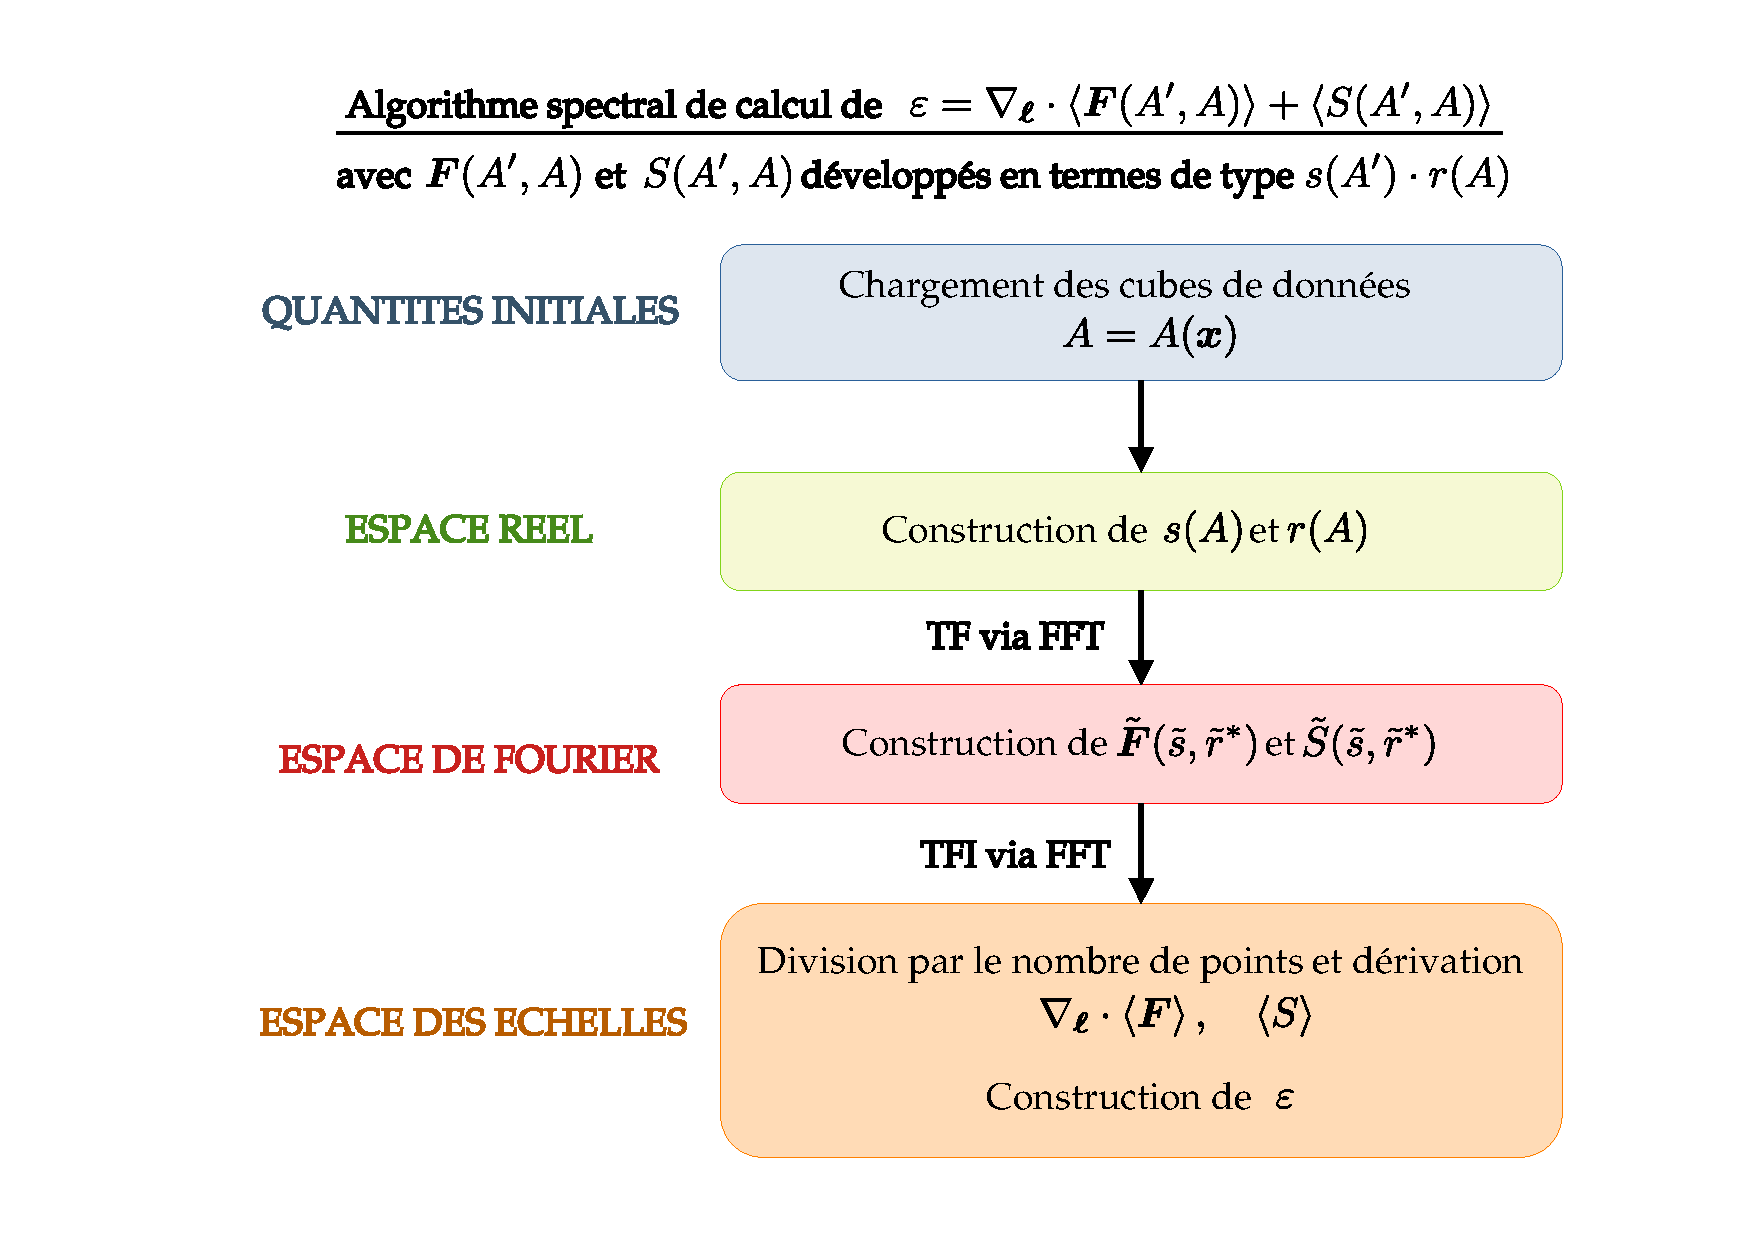
\includegraphics[width=0.93\linewidth,trim=4cm 1cm 3cm 1cm, clip=true]{./Mainmatter/Part_3/images_ch1/code_EL_spec}
 \cprotect\caption{Algorithme de calcul du taux de cascade \ensuremath{\varepsilon} via la convolution. Les quantités impliquées sont des quantités génériques.}
 \label{fig:algo_spec}
 \end{figure}
 Il demande quelques précautions lors de son implémentation, car il peut vite devenir coûteuse en mémoire, l'ensemble des termes présents dans une loi exacte devant être développé. Cependant, elle permet d'obtenir un résultat complet, indépendant du mode de représentation final des résultats. C'est donc la méthode qui a été choisie. De plus, en usant de l'algorithme de \cacro{FFT}, elle s'avère particulièrement rapide (moins de dix minutes pour calculer séparément les trois termes de \cacro{PP98} pour CGL2 par exemple).
 
 \section{Mode de représentation du résultat}
 \label{sec-313}
 \begin{figure}[!ht]
  \centering
 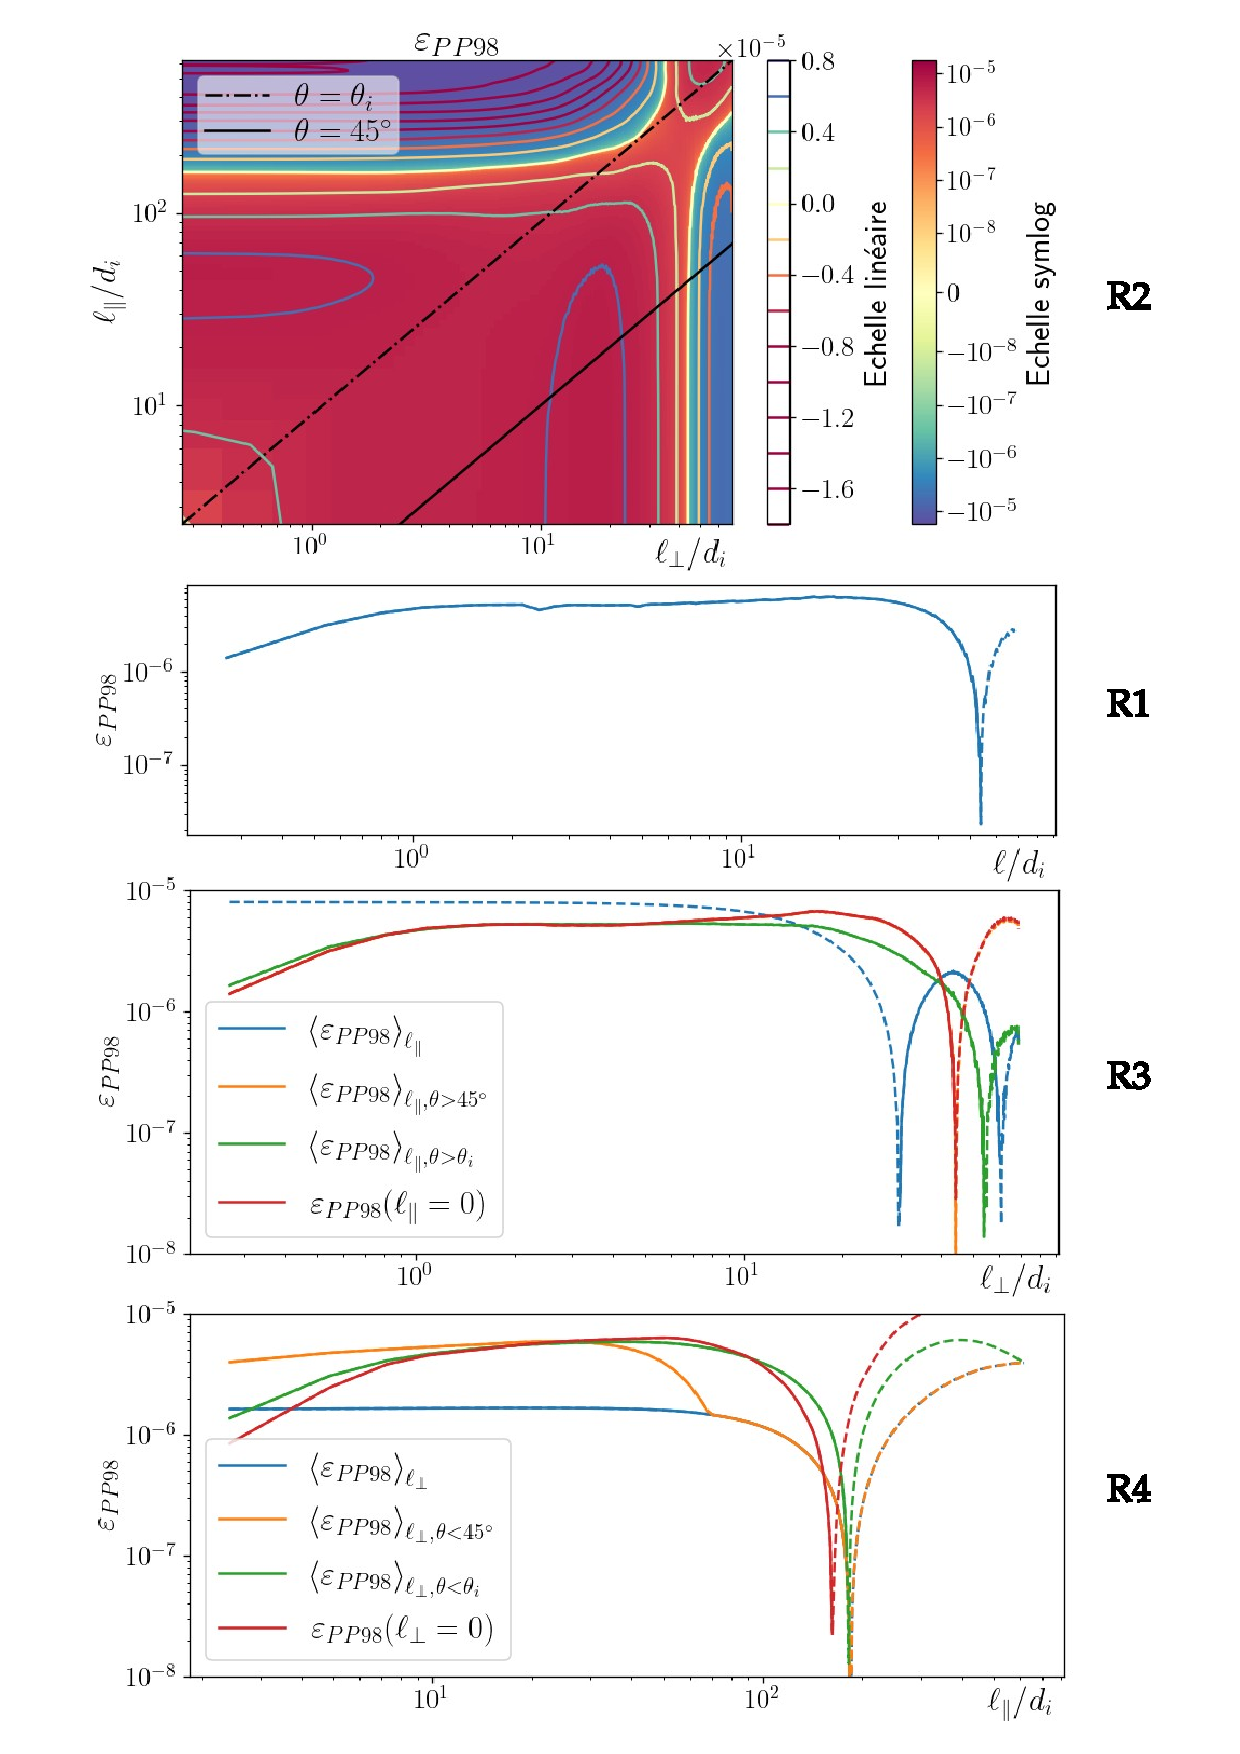
\includegraphics[width=0.75\linewidth,trim=1cm 0.5cm 1cm 0.5cm, clip=true]{./Mainmatter/Part_3/images_ch1/rep_CGL1}
 \cprotect\caption{Différents modes de représentations du taux de cascade \ensuremath{\varepsilon_{PP98}} calculé avec \cacro{PP98} dans les données de la simulation CGL1. R2 : \cacro{2D} en fonction de \ensuremath{\ell_{\perp}} et \ensuremath{\ell_{\parallel}}, avec deux échelles de couleurs, une échelle symlog, linéaire entre \ensuremath{-10^{-8}} et \ensuremath{10^{-8}} (barre de couleur continue), et une échelle linéaire (barre de couleur discontinue) et les frontières \ensuremath{\theta = \theta_i} (noire discontinue) et \ensuremath{\theta = \ang{45}} (noire continue). R1 : \cacro{1D} en fonction de \ensuremath{\ell}. R3 : \cacro{1D} en fonction de \ensuremath{\ell_{\perp}}, pour \ensuremath{\ell_{\parallel} = 0} (rouge), moyenne sur l'ensemble des \ensuremath{\ell_{\parallel}} (bleue), moyennes sur les \ensuremath{\ell_{\parallel}} tels que \ensuremath{\theta > \ang{45}} (orange) et \ensuremath{\theta > \theta_i} (vert). R4 : \cacro{1D} en fonction de \ensuremath{\ell_{\parallel}}, pour \ensuremath{\ell_{\perp} = 0} (rouge), moyenne sur l'ensemble des \ensuremath{\ell_{\perp}} (bleue), moyenne sur les \ensuremath{\ell_{\perp}} tels que \ensuremath{\theta < \ang{45}} (orange) et \ensuremath{\theta < \theta_i} (vert). Le caractère continu ou discontinu des courbes \cacro{1D} reflète le signe de \ensuremath{\varepsilon_{PP98}}.}
 \label{fig:rep_CGL1}
 \end{figure}
 Le résultat de l'algorithme de calcul par convolution est, pour chaque quantité, un parallélépipède couvrant une gamme d'échelles physiques dans la direction $\boldsymbol{e_z}$ différente de la gamme d'échelles couverte dans les directions perpendiculaires, $\boldsymbol{e_x}$ ou $\boldsymbol{e_y}$.  
 Ces gammes d'échelles couvrant différents ordres de grandeur, une représentation logarithmique est usuellement adoptée. Le caractère tridimensionnel de la grille parallélépipédique impose de choisir une méthode de réduction (\cacro{3D} vers \sacro{2D} ou \cacro{1D}) afin de pouvoir visualiser facilement les quantités. Différents types de réduction sont possibles et illustrés sur la \figref{fig:rep_CGL1} : 
 
\begin{itemize}
    \item R1 : \cacro{1D} en fonction de $\ell = |\boldsymbol{\ell}|$, en moyennant la quantité sur des coquilles de rayon moyen $\ell$,
    \item R2 : \sacro{2D} en fonction de $\ell_{\perp} = \sqrt{\ell_x^2 + \ell_y^2}$ et $\ell_{\parallel} = \ell_z$, en moyennant la quantité sur des couronnes de rayon moyen $\ell_{\perp}$ dans chaque plan perpendiculaire à $\boldsymbol{e_z}$,
    \item R3 : \cacro{1D} en fonction de $\ell_{\perp}$, en moyennant la quantité sur des coquilles cylindriques de rayon moyen $\ell_{\perp}$, la moyenne suivant $\ell_{\parallel}$ peut s'effectuer de diverses manières qui seront détaillées par la suite,
    \item R4 : \cacro{1D} en fonction de $\ell_{\parallel}$ en moyennant chaque plan perpendiculaire à $\boldsymbol{e_z}$, la moyenne suivant $\ell_{\perp}$ peut s'effectuer de diverses manières qui seront détaillées par la suite. 
\end{itemize}
 
 Sachant que la grille parallélépipédique couvre des gammes d'échelles différentes dans la direction $\boldsymbol{e_z}$ et les directions perpendiculaires (voir la carte R2 sur la \figref{fig:rep_CGL1}), notre géométrie est fondamentalement axisymétrique. La représentation de type R2 est donc la plus adaptée. L'échelle \og symlog \fg{}\footnote{Cette échelle décrit l'ensemble des nombres réels via trois représentations : $[x_0;+\infty[$ en représentation logarithmique, $]-x_0;x_0[$ en représentation linéaire (afin d'éviter la singularité du point 0), puis  $]-\infty; -x_0]$ en représentation logarithmique (en prenant l'opposé du logarithme de la valeur absolue). $x_0$ est choisi le plus petit possible.} permet de repérer les changements de signe et les ordres de grandeur couverts par $\varepsilon_{PP98}$ tandis que les courbes de niveau linéaires révèlent les variations plus spécifiques telles qu'un affaiblissement aux petites échelles ou des bosses (courbes de niveau bleues) aux échelles parallèles et perpendiculaires intermédiaires. On pourrait définir une zone inertielle entre les courbes de niveau associées à la valeur $\num{0.4}$. On remarque que cette zone semble carrée, cela est dû aux axes logarithmiques. Avec des axes linéaires, on observerait un quart d'ellipse liant $\ell_{\parallel}/d_i = \num{1e2}$ à $\ell_{\perp}/d_i \simeq \num{30} $. Le problème des cartes est la difficulté de comparer de multiples quantités. Une représentation \cacro{1D} sera donc nécessaire.

 R1 peut donner un résultat biaisé. Ainsi, sur le graphique R1 de la \figref{fig:rep_CGL1}, le résultat correspond quasiment entièrement (sauf aux très grandes échelles communes aux directions parallèle et perpendiculaire) à $\varepsilon_{PP98} (\ell_{\parallel} = 0)$ (en rouge sur le graphique R3 de la \figref{fig:rep_CGL1}). Le manque de points pour effectuer la moyenne en chaque $\ell$, induit des variations non-physiques du résultat (sursauts à intervalles réguliers sur le graphique R1 de la \figref{fig:rep_CGL1}). R3 ou R4 sont peut-être plus adaptés même si le caractère petit ou grand des échelles est défini à partir de $\ell=|\boldsymbol{\ell}|$ (resp. petit ou grand). 
 
 Cependant, visualiser la cascade via R3 en moyennant l'ensemble des $\ell_{\parallel}$ à $\ell_{\perp}$ fixé (courbe bleue) vient mixer les petits et grands $\ell$. La zone négative à grand $\ell_{\parallel}$ vient alors écraser la zone inertielle présumée et plus encore la variation des petites échelles. Le même phénomène apparaît pour R4 (courbes bleues sur les graphiques R3 et R4 de la \figref{fig:rep_CGL1}). Une autre possibilité de réduction serait de ne regarder qu'une direction $\ell_{\parallel} = 0$ pour R3 ou $\ell_{\perp} = 0$ pour R4 (courbes rouges sur les graphiques R3 et R4 de la \figref{fig:rep_CGL1}). Le résultat n'est alors pas très lisse et peu représentatif de la variation d'ensemble. 

 La troisième possibilité correspond à appliquer un filtre angulaire. En définissant $\theta$, l'angle entre $\boldsymbol{\ell}$ et $\boldsymbol{e_z}$, on pourrait considérer que les $\boldsymbol{\ell}$ contribuant à la dynamique parallèle sont les $\boldsymbol{\ell}$ quasi-parallèles tels que $\theta < \ang{45}$, et ceux contribuant à la dynamique perpendiculaire les $\boldsymbol{\ell}$ quasi-perpendiculaires tels que $\theta < \ang{45}$. La frontière $\theta = \ang{45}$ est représentée par une ligne noire continue sur la carte R2 de la \figref{fig:rep_CGL1}, et les résultats apparaissent en orange sur les graphiques R3 et R4. Pour R3, le résultat coïncide avec $\varepsilon_{PP98} (\ell_{\parallel} = 0)$. En effet, aux petites échelles, le plan tel que $\ell_{\parallel} = 0$ est la seule contribution à la moyenne. Similairement, pour R4, on assiste à un écroulement de la courbe qui rejoint $\left< \varepsilon_{PP98} \right>_{\ell_{\perp}}$ en $\ell_{\parallel} = \num{7e1}$. Cet écroulement est dû à la prise en compte de la région bleue à droite de la carte R2 pour les échelles supérieures à $\num{7e1}$. Ce filtre angulaire n'est donc pas adapté.
 
 La réduction \cacro{1D} qui sera adoptée par la suite correspond à un filtrage angulaire basé sur l'angle d'injection de l'énergie $\theta_i$. Ce dernier impose la géométrie de la grille et les gammes d'échelles accessibles. Dans l'espace des échelles, l'injection a lieu aux échelles telles que $\ell$ est maximal, c'est-à-dire dans l'angle supérieur droit de la carte R2 \figref{fig:rep_CGL1}. $\theta = \theta_i$ correspond à la diagonale représentée par une ligne noire discontinue. Appliquer cette réduction nous donne les courbes vertes des graphiques R3 et R4 de la \figref{fig:rep_CGL1}. N'y apparaissent, ni les artéfacts visibles avec R1, ni les saturations visibles sur les courbes bleues ou oranges, et elles sont plus représentatives du comportement de $\varepsilon_{PP98}$ dans l'ensemble de l'espace des échelles que les courbes rouges. On remarquera tout de même que la décroissance en allant vers les petites échelles est moins accentuée que pour les courbes rouges : les premières échelles de $\ell_{\parallel}$ (resp. $\ell_{\perp}$) différentes de $\num{0}$ sont prises en compte dans la moyenne des premiers points de $\varepsilon_{PP98}$ en fonction de $\ell_{\perp}$ (resp. $\ell_{\parallel}$).
 
%\newpage
 \section{Synthèse des méthodes et choix numériques}
 \label{synt-31}
\fcolorbox{blue}{white}{\begin{minipage}[c]{\linewidth}

\paragraph{\\Code de simulation d'un plasma turbulent (\texttt{Fortran}) : }
\begin{itemize}
\item Méthode d'intégration pseudo-spectrale (voir \figref{fig:algo_OCA}) des équations fluides.
\item Des termes d'hyperdissipation qui joueront le rôle de la dissipation aux petites échelles.
\item Un forçage permanent (dans l'espace de Fourier) de fréquences aléatoires proches de la pulsation Alfvénique et maintenant l'énergie perpendiculaire (cinétique + magnétique) du système quasiment constante.
\item Une géométrie périodique dépendant de l'angle d'injection de l'énergie $\theta_i$ et de la résolution de la grille numérique. \\
\end{itemize}
Je n'ai pas participé à l'écriture de ce code mais je l'ai utilisé pour compléter le lot de simulations analysé par \cite{ferrand_fluid_2021}.
\end{minipage}}

\fcolorbox{red}{white}{\begin{minipage}[c]{\linewidth}
\paragraph{\\Calcul des termes des lois exactes (\texttt{Python/Numpy/Scipy}) : }
Obtention rapide de {\bf l'ensemble de l'espace d'échelles accessible} grâce à une méthode de calcul spectrale basée sur le lien entre corrélation et convolution et sur la périodicité des simulations. L'algorithme est schématisé sur la \figref{fig:algo_spec}.

\paragraph{\\Visualisation des résultats (\texttt{Python/Matplotlib}) : représentation cylindrique} 
\begin{itemize}
\item Représentation \sacro{2D} en fonction de $\ell_{\parallel}$ et $\ell_{\perp}$ avec des échelles de couleurs de type chaud/froid (indiquant facilement le signe du résultat) associées aux variations logarithmiques (fond) et linéaires (courbes de niveaux) du résultat. 
\item Représentation \cacro{1D} en fonction de $\ell_{\perp}$. Réduction du résultat \sacro{2D} en moyennant sur $\ell_{\parallel}$ pour $\theta > \theta_i$.
\item Représentation \cacro{1D} en fonction de $\ell_{\parallel}$. Réduction du résultat \sacro{2D} en moyennant sur $\ell_{\perp}$ pour $\theta < \theta_i$. 
\end{itemize} 
Avec $\theta$ l'angle entre $\boldsymbol{\ell}$ et la direction moyenne du champ magnétique $\boldsymbol{e_z}$. \\

J'ai implémenté les codes de post-traitement et de visualisation des termes des lois exactes. Le code de post-traitement est disponible sur [GitHub : \cite{noauthor_paulinesimon972022-07_simu_exact_laws_nodate}].
\end{minipage}}

